%% LocalSeek: manuscript for Personal and Ubiquitous Computing (Springer Nature LaTeX template, version 3.1, Dec 2024).
%% Build: pdflatex main; bibtex main; pdflatex main; pdflatex main   (or: latexmk -pdf main.tex)
%% Figures: figures/*.pdf (charts) and drawio/*.pdf (diagrams exported from the Mermaid sources in diagrams/*.mmd).
\documentclass[pdflatex,sn-basic,Numbered]{sn-jnl}

\usepackage{graphicx}%
\usepackage{multirow}%
\usepackage{amsmath,amssymb,amsfonts}%
\usepackage{xcolor}%
\usepackage{textcomp}%
\usepackage{manyfoot}%
\usepackage{booktabs}%
\usepackage{tabularx}%
\usepackage[section]{placeins}%


\renewcommand{\topfraction}{0.85}
\renewcommand{\bottomfraction}{0.6}
\renewcommand{\textfraction}{0.12}
\renewcommand{\floatpagefraction}{0.8}
\setcounter{topnumber}{3}
\setcounter{bottomnumber}{2}
\setcounter{totalnumber}{4}
\newcommand{\ndcg}{nDCG@10}

\raggedbottom

\begin{document}

\title[LocalSeek: Private Hybrid Search for Android Smartphones]{LocalSeek: Private Hybrid Search for Android Smartphones}

\author*[1]{\fnm{Greenal Rajkumar} \sur{Tambe}}\email{greenaltambe1@gmail.com}
\author[1]{\fnm{Parikshit} \sur{Patil}}
\author[1]{\fnm{Kartik} \sur{Thakur}}
\author[1]{\fnm{Archit} \sur{Utsahi}}

\affil*[1]{\orgname{Sardar Patel Institute of Technology}, \orgaddress{\city{Mumbai}, \state{Maharashtra}, \country{India}}}

\abstract{Searching a phone's own files, apps and contacts should happen on the device, yet there is little published evidence on how to build such a search engine, because personal collections cannot be shared. We present LocalSeek, an open-source Android app that combines lexical BM25 ranking with dense retrieval from a small sentence-embedding model and needs no network permission, and we evaluate it in three studies. In a pre-registered study on one owner's phone (77 scored real-use queries, nine configurations), a hybrid of exact dense search and rank fusion reached a normalised discounted cumulative gain at rank 10 (nDCG@10) of 0.838, 0.254 above BM25 alone, and beat the configuration shipped during development by 0.147. Merging the ranks rather than the raw scores of three lexical tables gained 0.105. Locality-sensitive hashing and cross-encoder reranking showed no detectable benefit, and reranking cost 4.8 s per query. On eleven volunteers' own phones, with blind judging, the hybrid again led BM25 (+0.194) and dense search alone (+0.067); both gains were significant only in a sensitivity analysis that included every volunteer. Benchmarks on two phones with up to 200,000 vectors show that exact search is fast at personal scale and that a binary shortlist with rescoring finds at least 97.5\% of the true top 10 in under 30 ms beyond it, while the former hashing index found only 3 to 13\% of the true neighbours. A replication on five public datasets confirms the cost of hashing and the absence of a reranking gain.}

\keywords{On-device search, Hybrid retrieval, Personal information retrieval, Dense retrieval, Mobile computing, Pre-registration}

\maketitle

%=====================================================================
\section{Introduction}

A smartphone holds documents, installed apps, contacts and photos, and people expect one search box to find any of them. Sending that collection to a server raises privacy and availability concerns, so the search engine has to run on the phone itself. Small sentence-embedding models now run on phones, which makes it practical to combine lexical retrieval (BM25) with dense retrieval on the device.

The design space is large: which retrievers to combine, how to fuse their rankings, whether to rerank, and which nearest-neighbour index to use for the dense half. Most guidance on these choices comes from web and question-answering benchmarks with millions of documents. A personal collection differs in three ways. It is small (here about 13,700 text chunks plus about 100 apps and 200 contacts). It mixes several kinds of items. And it cannot be shared, so the community has few test collections for it \citep{kim2009pseudodesktop}.

We built LocalSeek, an Android app that searches files, apps, contacts and images with no network permission. During development the app shipped with an approximate dense index based on random-projection LSH, score-normalised fusion, result diversification and a rule that skipped dense search when BM25 looked confident. The question this paper answers is: \emph{which of these choices actually help, and which hurt, at the scale of one person's phone?} We answer it with three studies (Figure~\ref{fig:studies}):
\begin{enumerate}
  \item \textbf{Study 1: retrieval quality on real phones.} Part~1A (confirmatory) is a pre-registered evaluation on the owner's phone with 95 real-use queries, nine configurations, five hypotheses and a cluster-level analysis. Part~1B (exploratory, planned in advance) repeats the central comparison of BM25, dense and hybrid search on eleven volunteers' own phones, with blind judging (Sections~\ref{sec:s1method} and~\ref{sec:s1results}).
  \item \textbf{Study 2: speed and cost (descriptive).} A scaling microbenchmark of exact, quantised, LSH and HNSW search on two phones from 10,000 to 200,000 vectors, resource use, and search latency and index build time on the eleven volunteers' phones (Section~\ref{sec:s2}).
  \item \textbf{Study 3: replication on public data (exploratory).} The app pipeline ported to Python and run on five public BEIR datasets, with an analysis plan committed before any result, and a comparison of five small embedding models (Section~\ref{sec:s3}).
\end{enumerate}

\begin{figure}[tbp]
\centering
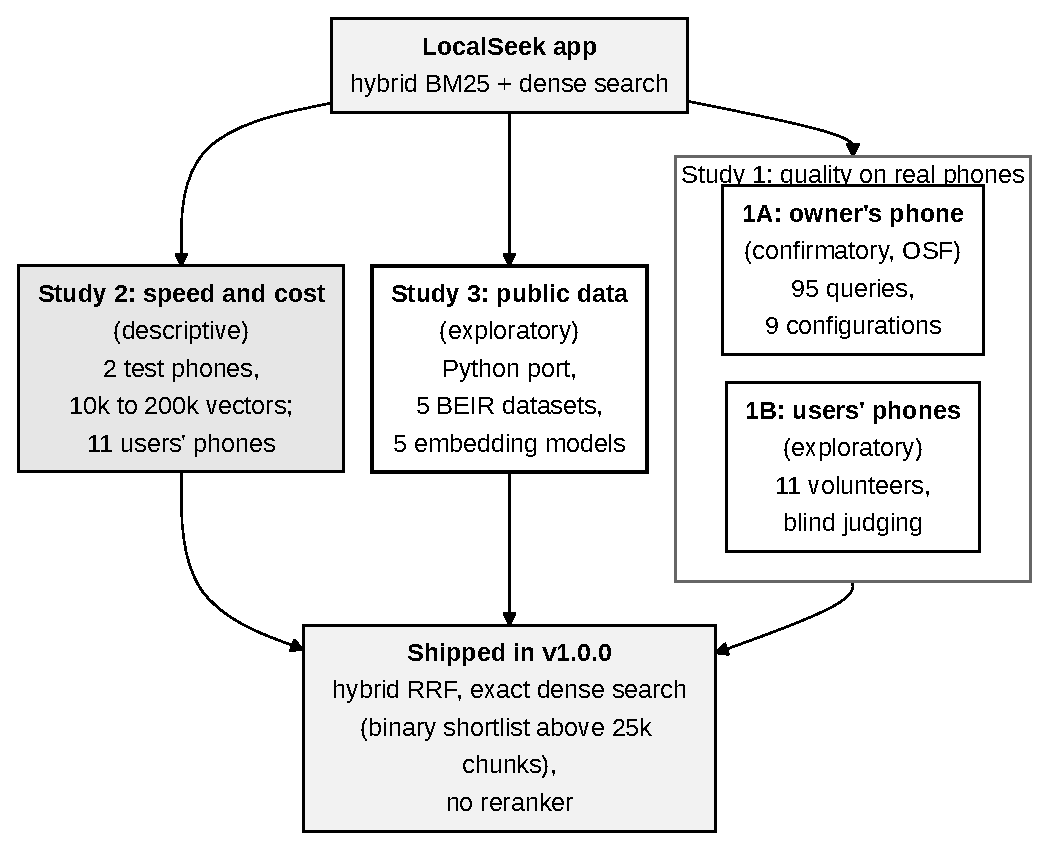
\includegraphics[width=\linewidth]{Fig1.pdf}
\caption{The three studies and how they feed the configuration that version 1.0.0 ships. Study 1 tests retrieval quality on real phones: confirmatory on the owner's phone (1A) and on eleven volunteers' own phones (1B). Study 2 checks speed and cost at larger sizes and on other phones; Study 3 asks whether the quality findings hold on data anyone can download}
\label{fig:studies}
\end{figure}

Besides the app itself (Section~\ref{sec:system}), the contributions are:
\begin{itemize}
  \item Evidence that, at personal scale, \textbf{exact dense search is fast enough on a phone} and the LSH index loses most true neighbours; the quality loss from LSH is significant on all five public datasets.
  \item A \textbf{pre-registered on-device evaluation}, rare in information retrieval. It shows the configuration shipped during development was 0.147 \ndcg{} below the best one available, and it reports its null results as nulls.
  \item A \textbf{multi-source merging artefact}: putting raw BM25 scores from several FTS5 tables on one min-max scale cost 0.105 \ndcg{} compared with merging their ranks.
  \item \textbf{Reranking with a cross-encoder did not pay} on the phone: no detectable gain in Study~1 or Study~3, at about 4.8\,s per query.
  \item \textbf{Practical guidance} measured on two test phones and eleven volunteers' phones: the collection size at which exact search stops being enough, and what to use beyond it.
  \item \textbf{Evidence from other users' phones}: on eleven volunteers' own collections, judged blind, the hybrid again led BM25 by about 0.2 \ndcg{} and dense search by a small margin, with search latency, index build time and usability reported per phone.
  \item An \textbf{open-source app, harness and analysis code}, with the confirmatory analysis scripts frozen by commit.
\end{itemize}

%=====================================================================
\section{Related work}

\paragraph{Personal and desktop search.} Stuff I've Seen showed that people re-find their own material through a single index across sources \citep{dumais2003sis}. Evaluating such systems is hard because the collections are private; \citet{kim2009pseudodesktop} built pseudo-desktop collections to get around this. Our response is different: a pre-registered single-owner study that publishes only aggregates, paired with a study on eleven volunteers' own phones and a replication on public data.

\paragraph{Lexical, dense and hybrid retrieval.} BM25 \citep{robertson2009bm25} remains a strong baseline. Dense bi-encoders \citep{reimers2019sbert,karpukhin2020dpr} add semantic matching, and MiniLM \citep{wang2020minilm} is a common small encoder for phones. BEIR \citep{thakur2021beir} showed that neither family wins everywhere zero-shot, which motivates hybrids. Reciprocal-rank fusion \citep{cormack2009rrf} merges rankings without calibrating scores. \citet{bruch2023fusion} compared fusion functions and found that convex combinations of normalised scores can beat RRF when tuned; our Study~3 compares the app's RRF with its global score normalisation, untuned. Cross-encoder reranking \citep{nogueira2019bert} usually improves effectiveness at a large compute cost.

\paragraph{Nearest-neighbour search.} Random-projection LSH \citep{indyk1998lsh,charikar2002simhash} hashes vectors into buckets. Graph indexes such as HNSW \citep{malkov2020hnsw} and quantisation \citep{jegou2011pq} dominate modern benchmarks \citep{aumuller2020ann,johnson2021faiss}. Binary codes followed by exact rescoring of a shortlist were shown to keep passage-retrieval quality at a fraction of the memory \citep{yamada2021bpr}. These results come from server-scale collections; Studies~2 and~3 ask what matters at about $10^4$ to $10^5$ vectors on a phone.

\paragraph{On-device retrieval.} Recent work targets retrieval-augmented generation on edge devices. EdgeRAG prunes and generates embeddings on demand to fit memory \citep{seemakhupt2024edgerag}; MobileRAG proposes a mobile-friendly vector search, EcoVector, and compares it with IVF and HNSW variants \citep{park2025mobilerag}. These systems optimise the vector index for large collections; we evaluate retrieval quality end to end on a real personal collection and on public data.

\paragraph{Small embedding models.} BGE \citep{xiao2024cpack}, Arctic-Embed \citep{merrick2024arctic} and EmbeddingGemma \citep{vera2025embeddinggemma} target efficient retrieval; EmbeddingGemma supports Matryoshka truncation \citep{kusupati2022mrl}. Model2Vec distils static embeddings \citep{vandongen2024model2vec}. MTEB \citep{muennighoff2023mteb} compares such models on server hardware; we compare them inside the same hybrid pipeline.

\paragraph{Evaluation methodology.} We use \ndcg{} \citep{jarvelin2002ndcg} and bpref \citep{buckley2004bpref}. Paired randomisation tests are recommended for IR significance testing \citep{smucker2007significance}, with Holm's correction for families of tests \citep{holm1979}; confidence intervals come from the percentile bootstrap \citep{efron1993bootstrap}. Pre-registration separates confirmatory from exploratory results \citep{nosek2018prereg}. Using one assessor is a known source of variation in relevance judgments \citep{voorhees2000variations}.

%=====================================================================
\section{The LocalSeek system}\label{sec:system}

LocalSeek is an Android app written in Kotlin with Jetpack Compose (minimum Android 8.0, target API 36). It requests no INTERNET permission, and a build check fails if that permission ever appears in a merged manifest. App backups are disabled and everything is indexed and searched in app-private storage. Figure~\ref{fig:arch} shows the architecture.

\begin{figure}[tbp]
\centering
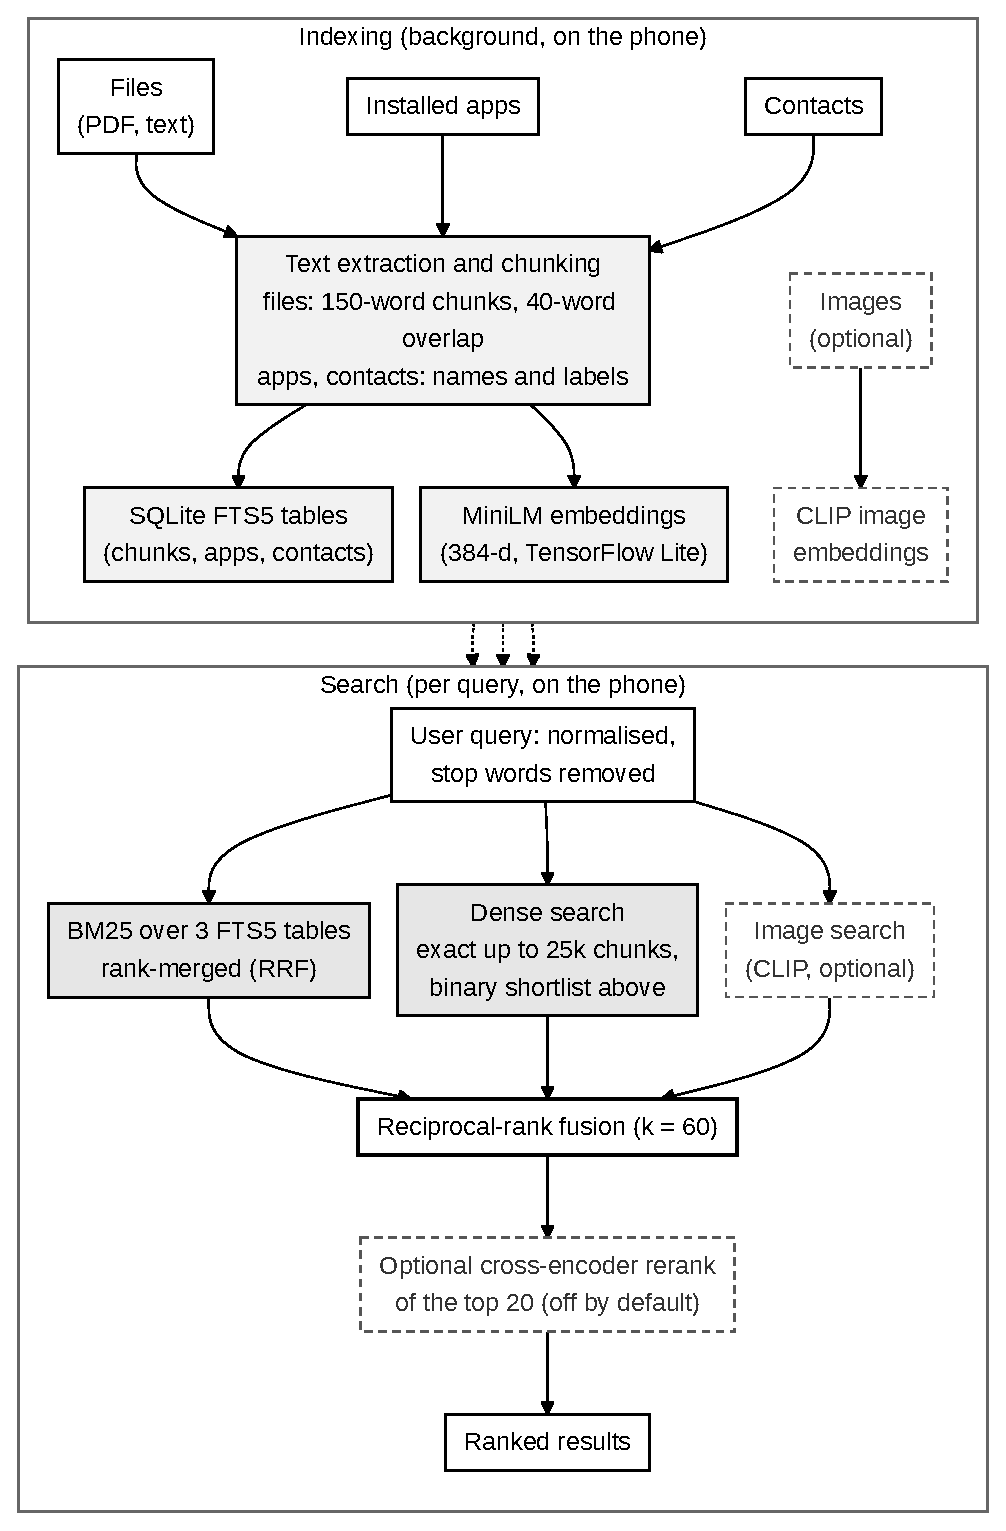
\includegraphics[width=0.85\linewidth]{Fig2.pdf}
\caption{LocalSeek architecture (version 1.0.0). In the background, indexers store text in SQLite FTS5 tables and MiniLM embeddings beside them. At query time BM25, dense and (optionally) image retrieval run, reciprocal-rank fusion (RRF) merges their lists, and an optional cross-encoder can rerank the top 20. Dashed boxes are optional and off in every experiment}
\label{fig:arch}
\end{figure}

\paragraph{Indexing.} Background workers index four kinds of items: \emph{files} (PDF text from the first 10 pages and plain-text formats from the first 100\,KB; Office formats are not indexed), \emph{apps} and \emph{contacts} (names and labels), and optionally \emph{images} with a CLIP ViT-B/32 model delivered as a separate asset pack. Images are excluded from every experiment in this paper. File text is split into chunks of 150 words with a 40-word overlap. Each chunk is stored in a SQLite FTS5 table through Room and embedded with all-MiniLM-L6-v2 \citep{wang2020minilm}: a 22.7\,MB TensorFlow Lite model, 384 dimensions, mean pooling, 128 tokens. Apps and contacts live in two further FTS5 tables and have their own embeddings.

\paragraph{Query processing and retrieval.} A query is normalised and stop-word filtered, and optionally expanded with synonyms. Two retrievers then run. \emph{BM25} uses FTS5's \texttt{bm25()} over the three tables, with a cascade from AND to OR queries. \emph{Dense} retrieval takes the cosine similarity between the query embedding and the chunk embeddings, keeping the top 50 chunks above a cosine of 0.3 and the best chunk per file. Apps and contacts are matched by FTS and by an exact scan of their embeddings, independent of the dense index used for file chunks. During development the dense half had three interchangeable indexes for file chunks: random-hyperplane \emph{LSH} (at the phone's collection size, 10 tables of 10 bits and a cap of 100 candidates; the battery level at build time could shrink this structure, see Section~\ref{sec:limits}), \emph{exact search} over the embeddings in the database, and \emph{exact search in memory} over a contiguous copy (about 21\,MB at this size).

\paragraph{Fusion and reranking.} Results are fused either by reciprocal-rank fusion (RRF, $k=60$, plus a title-match ranking) or by global min-max score normalisation. With $r_i(d)$ the rank of document $d$ in list $i$,
\begin{equation}
\mathrm{RRF}(d) = \sum_{i} \frac{1}{k + r_i(d)}.
\end{equation}
An optional cross-encoder (ms-marco-MiniLM-L-6-v2, 45\,MB in TensorFlow Lite) reranks the top candidates. Optional maximal-marginal-relevance diversification and a dense-skip rule complete the pipeline.

\paragraph{Shipped configurations.} Before this study the app shipped a configuration with these settings: battery-adaptive LSH, global score normalisation, diversification on, dense skip when the top BM25 score reached 0.85, query expansion on, and no reranking. Its benchmark replica is arm E12. After Study~1, version 1.0.0 ships arm E9 for text: hybrid RRF with exact in-memory dense search, no diversification, no dense skip and no reranking. Following Study~2, its dense index is size-adaptive: exact search up to 25,000 chunks and a binary shortlist with float rescoring ($k'=200$) above that. The threshold was first set at 50,000 from the first phone and lowered to 25,000 after the second, slower phone (Section~\ref{sec:s2}). At the owner's collection size (13,696 chunks) the exact path is used. The app no longer builds an LSH index; that code remains only for the benchmark arms. Unit tests assert that the shipped configuration equals E9 in every text-retrieval setting and that the size-adaptive index returns rankings identical to E9's below the threshold. A second test pins the configuration hash of all 18 benchmark arms, so the switch could not alter any registered arm.

\paragraph{Use of generative AI.} The authors used a large language model assistant (Claude, Anthropic) as a programming and writing aid: to write and review parts of the app and benchmark code and the analysis scripts, and to draft and edit the manuscript text. All analysis plans, hypotheses and design decisions were reviewed and approved by the authors before use; all code was reviewed and tested by the authors; every reported number was produced by the scripts in the repository and checked against their outputs; and the authors take full responsibility for the content.

%=====================================================================
\section{Study 1: method}\label{sec:s1method}

Study~1 measures retrieval quality on real phones in two parts. Part~1A is the confirmatory evaluation on one owner's phone, registered before any run. Part~1B repeats its central comparison (BM25, dense and hybrid search) on eleven volunteers' own phones, under a plan committed before any participant data existed. Part~1A has depth: nine configurations and 77 scored queries on one collection. Part~1B has breadth: eleven people, phones and collections, with fewer searches each.

\subsection{Study 1A: the owner's phone (pre-registered)}\label{sec:s1a}

\paragraph{Pilot and registration.} A pilot (Set~A: 64 queries, 60 scored, 12 configurations) revealed that the LSH arm lost 0.272 \ndcg{} against exact dense search (Holm $p<0.001$). That finding and other pilot observations shaped the confirmatory study. Set~A was seen before the design and is used only as disclosed pilot evidence. The confirmatory plan for a new query set, Set~B, was registered on OSF (\url{https://osf.io/vwmfz}) on 2026-10-04, before any Set~B run; the registered commit fixes the arms, hypotheses, stop rules and analysis scripts. Figure~\ref{fig:protocol} summarises the protocol.

\begin{figure}[tbp]
\centering
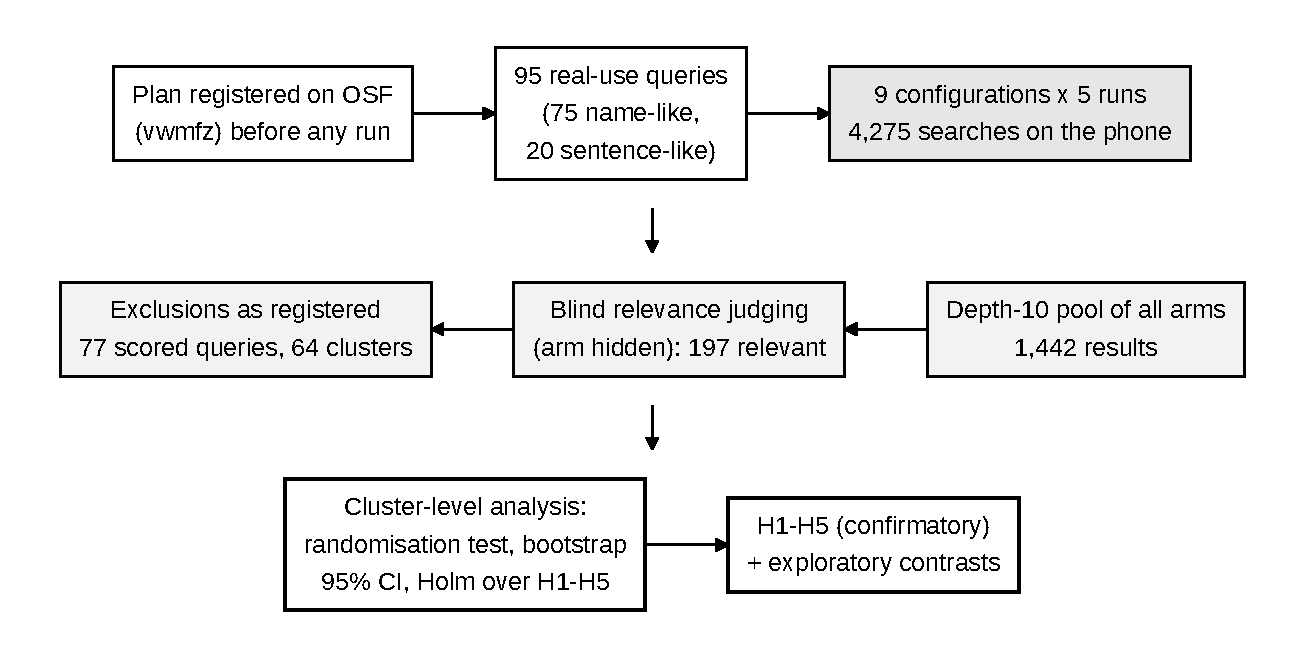
\includegraphics[width=\linewidth]{Fig3.pdf}
\caption{Study 1 protocol, from registration to the registered analysis. Numbers are those of the Set~B run}
\label{fig:protocol}
\end{figure}

\paragraph{Collection and device.} One owner's OnePlus phone (Android 16). At the run it held 13,696 text chunks, 97 apps, 189 contacts and 522 images (images were off in every arm), and the collection was frozen for the run. A script checked the run conditions: nominal LSH structure (10 tables, cap 100, 13,503 vectors) with an identical index hash before and after, thermal status NONE or LIGHT in every run, charging, airplane mode off, and identical collection counts at start and end.

\paragraph{Queries.} The owner wrote 95 queries from real use before any Set~B result existed: 75 name-like and 20 sentence-like. Of these, 79 target text items (47 files, 20 apps, 11 contacts, 1 typo) and 16 target images only, which are excluded as registered. Variants of one need share a cluster id. Two text queries had no relevant item and are excluded, which leaves \textbf{77 scored queries in 64 clusters}.

\paragraph{Arms.} Nine configurations (Table~\ref{tab:arms}), five repetitions each: 4,275 runs in 57 minutes.

\begin{table}[tbp]
\centering\footnotesize\setlength{\tabcolsep}{3pt}
\caption{The nine configurations (arms) of Study 1.}
\label{tab:arms}
\begin{tabularx}{0.9\linewidth}{lX}
\toprule
Arm & Configuration \\
\midrule
E1 & BM25 over three FTS5 tables, one min-max scale over raw scores \\
E1b & E1 with rank-based (RRF) merge of the three tables \\
E2 & Dense only, exact search \\
E3 & Dense only, LSH \\
E5 & Hybrid RRF, LSH dense \\
E9 & Hybrid RRF, exact in-memory dense (\emph{what version 1.0.0 ships}) \\
E10 & E9 plus cross-encoder rerank of the top 20 \\
E11 & E9 with the raw query sent to the dense encoder \\
E12 & Replica of the configuration shipped before the study \\
\bottomrule
\end{tabularx}
\end{table}

\paragraph{Judging.} A depth-10 pool over all arms was judged blind to arm, with binary relevance, by the owner: 1,442 rows, 197 of them relevant. A blind re-judge of 167 pooled rows (8 queries) by the same assessor, 166 of which were judged in both passes, gave Cohen's $\kappa=0.69$ (92.8\% raw agreement), which is substantial agreement on the usual Landis and Koch scale. Putting the second judgments in place of the first ones moved no arm mean by more than 0.01 and changed none of the five pre-registered conclusions.

\paragraph{Hypotheses.} Five contrasts on \ndcg{}: H1 E9 vs E5 (exact vs LSH in the hybrid), H2 E11 vs E9 (raw vs expanded dense query), H3 E1b vs E1 (table merging), H4 E10 vs E9 (reranking) and H5 E9 vs E12 (best evaluated vs shipped). A secondary analysis (S1, outside the Holm family) tests a confidence cascade that sends the two-thirds of queries with the smallest top-two score margin under E9 to E10; its three success criteria were fixed in advance.

\paragraph{Statistical analysis.} The unit of analysis is the cluster: the \ndcg{} values of the queries in one cluster are averaged first, so a need written in several words counts once. For each contrast we compute the per-cluster difference between the two arms on the same queries. Significance comes from a paired two-sided randomisation test (sign flips of the 64 cluster differences, 200,000 Monte Carlo samples) with Holm correction over the five contrasts. Each 95\% confidence interval is a percentile bootstrap: the 64 clusters are resampled with replacement 10,000 times with a fixed seed, the mean is recomputed each time, and the 2.5th and 97.5th percentiles are taken. The same procedure gives the intervals for the arm means, where the resampled value is the arm's own cluster mean rather than a difference. A per-query analysis (77 units) is reported as sensitivity. From the pilot's variance, the registration estimated the minimum detectable effect at about 0.06--0.07 \ndcg{}.

\subsection{Study 1B: other users' phones}\label{sec:s1b}

\paragraph{Participants and procedure.} Eleven volunteers from the authors' circle, each on their own Android phone, installed a study build of LocalSeek: a separate build type with no INTERNET permission, image search switched off and a consent screen. The Study~1A phone did not take part; one export from it was removed before the analysis, as the plan requires. Figure~\ref{fig:userstudy} shows the flow. Each volunteer let the app index their phone, then typed real searches for things they knew were on it (8 to 14 each, 106 in total; 10 to 15 were planned), and tagged each as a file, app or contact search and as keyword-like or sentence-like. For each search the app ran three arms of Study~1A unchanged: BM25 (E1), exact dense search (E2) and the shipped hybrid (E9). It merged the top 10 of each, removed duplicates, shuffled the list with a per-search seed and showed one list without arm labels, and the volunteer marked each item relevant or not. After about two minutes of free use, volunteers answered the 10-item System Usability Scale (SUS) \citep{brooke1996sus}. The app exports one file of numbers and enumerations. No search text, item name, identifier or path leaves the phone, and the analysis script rejects a file with any other text field.

\begin{figure}[tbp]
\centering
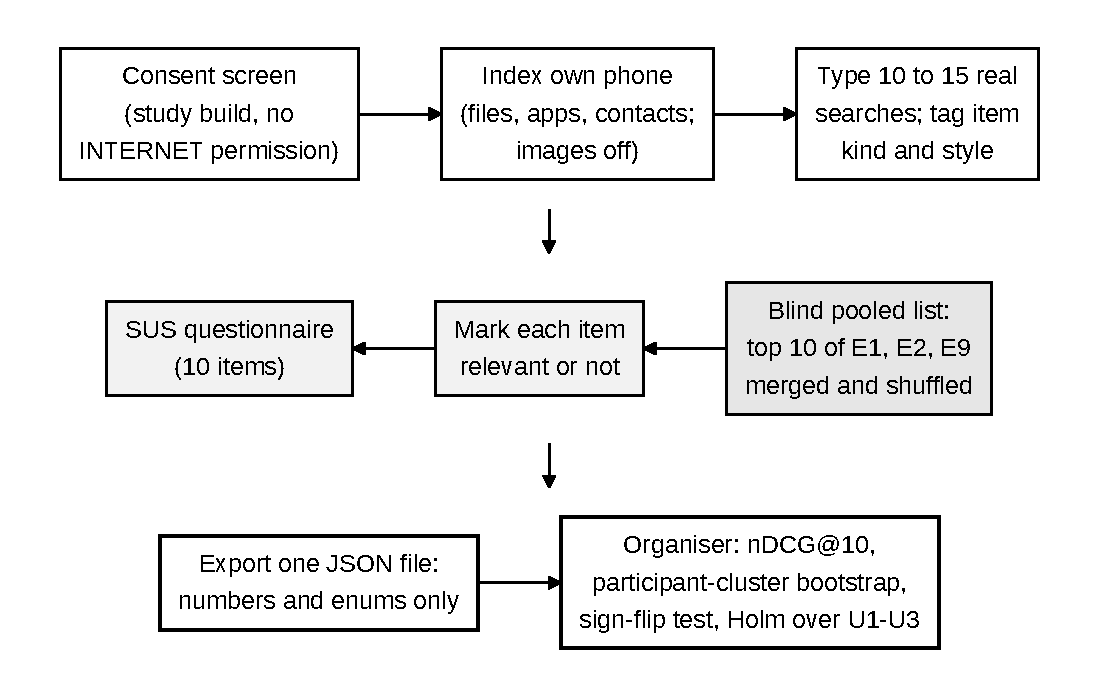
\includegraphics[width=\linewidth]{Fig4.pdf}
\caption{Study 1B flow on each volunteer's phone. Judging is blind to the method; the export holds numbers and enumerations only}
\label{fig:userstudy}
\end{figure}

\paragraph{Analysis plan.} The plan was committed to the repository before any participant file existed (commit \texttt{9a41587}). It was not registered on OSF, so Study~1B is exploratory. The metric is \ndcg{} with binary relevance, with the same definition as Study~1A: the ideal list contains all relevant items judged for that search. The contrasts are U1 E9 $-$ E1, U2 E9 $-$ E2 and U3 E2 $-$ E1. The unit is the participant. The 95\% interval is a participant-cluster percentile bootstrap: participants are resampled with replacement, then searches within each resampled participant (10,000 resamples, fixed seed). The $p$-value comes from an exact paired sign-flip test over the participants' mean differences (all $2^n$ sign patterns), Holm-corrected over U1 to U3. Searches with no relevant item are excluded. Participants with fewer than eight scored searches are excluded from the contrasts. With $n=6$ participants the smallest attainable two-sided $p$ is $2/2^6 = 0.031$, reached only when all six differences have the same sign. As a sensitivity analysis that was not in the plan, we repeat the contrasts with all eleven volunteers and every scored search.

%=====================================================================
\section{Study 1: results}\label{sec:s1results}

Sections~\ref{sec:s1hyp} to~\ref{sec:s1strata} report Study~1A on the owner's phone; Section~\ref{sec:s1bres} reports Study~1B on the volunteers' phones.

\subsection{Study 1A: registered hypotheses}\label{sec:s1hyp}

Two of the five registered hypotheses were significant: rank-based table merging (H3) and the best configuration over the shipped one (H5) (Table~\ref{tab:hyp}, Figure~\ref{fig:contrasts}).

\begin{table}[tbp]
\centering\footnotesize\setlength{\tabcolsep}{3pt}
\caption{Registered contrasts on \ndcg{}, cluster as the unit (64 clusters), Holm over five. The last column is the per-query sensitivity analysis (77 queries).}
\label{tab:hyp}
\begin{tabular}{llrlllr}
\toprule
H & Contrast & Diff. & 95\% CI & Holm $p$ & Verdict & By query \\
\midrule
H1 & E9 $-$ E5 (exact vs LSH in hybrid) & +0.044 & [$-$0.007, +0.095] & 0.285 & no evidence & +0.066$^{*}$ \\
H2 & E11 $-$ E9 (raw dense query) & +0.003 & [$-$0.008, +0.017] & 0.653 & no evidence & +0.004 \\
H3 & E1b $-$ E1 (RRF table merge) & +0.105 & [+0.039, +0.174] & 0.012 & \textbf{significant} & +0.076$^{*}$ \\
H4 & E10 $-$ E9 (rerank top 20) & +0.013 & [$-$0.011, +0.040] & 0.637 & no evidence & +0.017 \\
H5 & E9 $-$ E12 (best vs shipped) & +0.147 & [+0.080, +0.213] & 0.0002 & \textbf{significant} & +0.137$^{*}$ \\
\bottomrule
\multicolumn{7}{l}{\footnotesize $^{*}$ Holm $p<0.05$ in the per-query analysis (H1 0.038, H3 0.043, H5 $<$0.001).}
\end{tabular}
\end{table}

\begin{figure}[tbp]
\centering
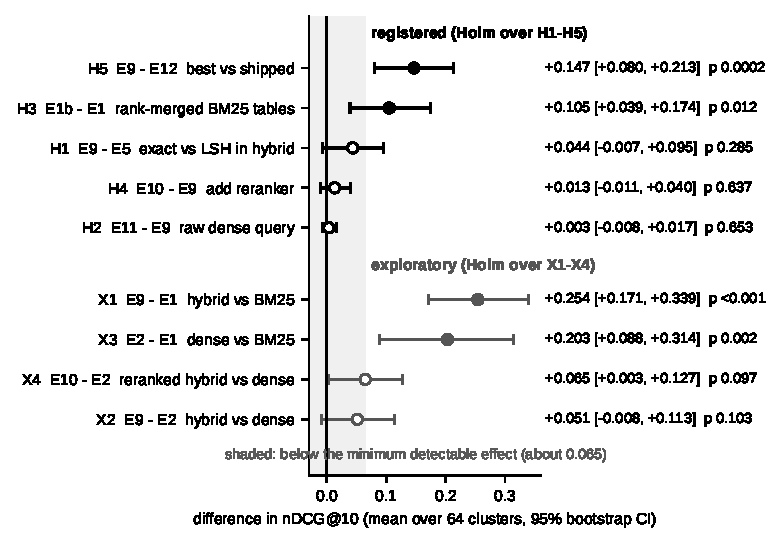
\includegraphics[width=\linewidth]{Fig5.pdf}
\caption{Study 1 contrasts as paired differences in \ndcg{} (cluster means, 95\% bootstrap CI). Filled markers: Holm-adjusted $p<0.05$ within their family (upper group: registered; lower group: exploratory). Shaded band: smaller than the registered minimum detectable effect}
\label{fig:contrasts}
\end{figure}

\paragraph{Analysis.} H5 is the largest registered effect: the shipped-before-study configuration lost 0.147 \ndcg{}, and the whole interval (+0.080 to +0.213) lies above the minimum detectable effect, so the loss is both significant and practically large. H3 shows that how the three lexical tables are merged matters as much as which retrievers are used: ranking them separately and merging by rank gained 0.105. H1, H2 and H4 are not significant. For H1 the point estimate favours exact search in both analyses, and the per-query analysis is significant (Holm $p=0.038$); as registered, the cluster-level result is the confirmatory one. H2 and H4 have narrow intervals around zero (at most $\pm$0.03), so any effect of query expansion or reranking on this collection is small.

\subsection{Study 1A: arm means and how to read the intervals}

\begin{table}[tbp]
\centering\footnotesize\setlength{\tabcolsep}{3pt}
\caption{Arm means and latency (descriptive). \ndcg{} by cluster with 95\% bootstrap CI; latency over 77 queries $\times$ 5 repetitions on the debug build (a release-mode build was 15--23\% faster, Section~\ref{sec:s2}).}
\label{tab:armmeans}
\begin{tabular}{lrlrrr}
\toprule
Arm & \ndcg{} & 95\% CI & bpref & Median (ms) & p95 (ms) \\
\midrule
E10 & 0.852 & [0.794, 0.905] & 0.744 & 4,774 & 4,968 \\
E11 & 0.842 & [0.790, 0.892] & 0.712 & 145 & 274 \\
E9 & 0.838 & [0.781, 0.890] & 0.710 & 145 & 282 \\
E5 & 0.795 & [0.728, 0.857] & 0.663 & 112 & 256 \\
E2 & 0.787 & [0.714, 0.856] & 0.678 & 312 & 354 \\
E12 & 0.692 & [0.616, 0.762] & 0.497 & 105 & 198 \\
E1b & 0.689 & [0.622, 0.753] & 0.472 & 44 & 225 \\
E1 & 0.584 & [0.500, 0.668] & 0.419 & 42 & 219 \\
E3 & 0.517 & [0.409, 0.627] & 0.477 & 97 & 118 \\
\bottomrule
\end{tabular}
\end{table}

\paragraph{Analysis.} The arm intervals in Table~\ref{tab:armmeans} are 0.11 to 0.22 wide, and they overlap for most pairs of arms. This width does not mean the comparisons are weak. An arm interval reflects how much \ndcg{} varies from one query to another: some needs are found at rank 1 by every arm and others are hard for all of them. When two arms are compared on the same clusters, that shared difficulty cancels, so the interval of the paired difference is much narrower. For example, the intervals of E1b and E1 overlap (0.622--0.753 and 0.500--0.668), yet their paired difference is +0.105 with an interval of [+0.039, +0.174] that excludes zero. For this reason we draw the comparisons as paired differences (Figure~\ref{fig:contrasts}) rather than as overlapping arm intervals. The intervals can only be made shorter honestly by judging more queries, not by changing the method; with 64 clusters, a half-width of about 0.05--0.06 for an arm mean corresponds to a between-cluster standard deviation of about 0.2 \ndcg{}, as expected for binary relevance.

E9 costs about 40\,ms more than E12 at the median and stays well inside an interactive budget; every arm without reranking has a p95 below 360\,ms, while the reranker raises the median to 4.8\,s.

\subsection{Study 1A: hybrid versus its parts (exploratory, not registered)}

The registration did not test the hybrid against its single retrievers. We computed these contrasts after the registered results were known, from the same runs, with the same cluster-level method and Holm over these four only (Table~\ref{tab:hybrid}, lower half of Figure~\ref{fig:contrasts}).

\begin{table}[tbp]
\centering\footnotesize\setlength{\tabcolsep}{3pt}
\caption{Hybrid versus single retrievers, \ndcg{}, 64 clusters (exploratory; Holm over these four).}
\label{tab:hybrid}
\begin{tabular}{lrlll}
\toprule
Contrast & Diff. & 95\% CI & Holm $p$ & By query (Holm $p$) \\
\midrule
E9 $-$ E1 (hybrid vs BM25) & +0.254 & [+0.171, +0.339] & $<$0.001 & +0.224 \\
E2 $-$ E1 (dense vs BM25) & +0.203 & [+0.088, +0.314] & 0.002 & +0.175 \\
E9 $-$ E2 (hybrid vs dense) & +0.051 & [$-$0.008, +0.113] & 0.103 & +0.050 (0.091) \\
E10 $-$ E2 (reranked hybrid vs dense) & +0.065 & [+0.003, +0.127] & 0.097 & +0.067 (0.058) \\
\bottomrule
\end{tabular}
\end{table}

\paragraph{Analysis.} Adding dense retrieval to BM25 is the single largest improvement measured (+0.254), and dense search alone already captures most of it (+0.203 over BM25). The hybrid's edge over dense search alone (+0.051) is positive in both analyses but not distinguishable from zero, and it is below the minimum detectable effect, so this study cannot say whether BM25 adds to dense search on this collection. The Set~A pilot points the same way (hybrid vs dense +0.066, CI [$-$0.022, +0.162]).

\subsection{Study 1A: ablation study}

An ablation study removes or changes one component of a system at a time and measures the effect, to show what each component contributes. Because every arm of Study~1 is an explicit configuration run on the same queries, the arms already form an ablation of the shipped pipeline E9 without any extra runs. Table~\ref{tab:ablation} lists each change relative to E9, with its effect on \ndcg{} and whether the comparison was registered in advance or computed afterwards.

\begin{table}[tbp]
\centering\footnotesize\setlength{\tabcolsep}{3pt}
\caption{Component ablation of the shipped pipeline E9 on Study 1 (\ndcg{} change relative to E9 unless stated).}
\label{tab:ablation}
\begin{tabular}{lrll}
\toprule
Change & $\Delta$\ndcg{} & Holm $p$ & Status \\
\midrule
Remove dense retrieval (BM25 only, E1) & $-$0.254 & $<$0.001 & exploratory \\
Remove BM25 (dense only, E2) & $-$0.051 & 0.103 & exploratory \\
Exact $\rightarrow$ LSH dense index (E5) & $-$0.044 & 0.285 & registered (H1) \\
Add cross-encoder rerank (E10) & +0.013 & 0.637 & registered (H4)\footnotemark[1] \\
Raw instead of expanded dense query (E11) & +0.003 & 0.653 & registered (H2) \\
Revert to pre-study shipped settings (E12) & $-$0.147 & 0.0002 & registered (H5) \\
RRF table merge, BM25 only (E1b vs E1) & +0.105 & 0.012 & registered (H3) \\
\bottomrule
\end{tabular}
\footnotetext[1]{at about 4.8\,s median latency per query instead of 0.15\,s.}
\end{table}

\paragraph{Analysis.} The ablation separates the components into three groups. \emph{Essential:} dense retrieval, whose removal costs 0.254 \ndcg{}, and rank-based merging of the lexical tables (+0.105 for BM25 alone). \emph{Helpful but not proven at this sample size:} BM25 alongside dense retrieval ($-$0.051 when removed) and the exact dense index ($-$0.044 when replaced by LSH; significant on all five public datasets in Study~3). \emph{Not worth their cost:} the cross-encoder reranker (+0.013 at about 30 times the latency) and query expansion for dense search (using the raw query instead changed \ndcg{} by only +0.003). Restoring all the settings shipped before the study at once costs 0.147 \ndcg{}.

\subsection{Study 1A: query types, item types and the cascade}\label{sec:s1strata}

\begin{table}[tbp]
\centering\footnotesize\setlength{\tabcolsep}{3pt}
\caption{Descriptive breakdowns (registered without tests). Left: registered contrasts by query style, cluster as the unit. Right: arm means by item type.}
\label{tab:strata}
\begin{tabular}{lll}
\toprule
Contrast & Name-like (57 clusters) & Sentence-like (17 clusters) \\
\midrule
H1 E9 $-$ E5 & +0.034 [$-$0.019, +0.086] & +0.168 [+0.059, +0.284] \\
H2 E11 $-$ E9 & +0.000 [$-$0.007, +0.007] & +0.015 [$-$0.023, +0.062] \\
H3 E1b $-$ E1 & +0.143 [+0.079, +0.214] & $-$0.133 [$-$0.227, $-$0.052] \\
H4 E10 $-$ E9 & +0.005 [$-$0.018, +0.031] & +0.055 [+0.004, +0.119] \\
H5 E9 $-$ E12 & +0.174 [+0.108, +0.241] & +0.029 [$-$0.078, +0.131] \\
\bottomrule
\end{tabular}\hfill
\begin{tabular}{lrrr}
\toprule
Arm & Apps & Contacts & Files \\
\midrule
E1 & 0.375 & 0.596 & 0.707 \\
E2 & 0.848 & 0.965 & 0.691 \\
E3 & 0.875 & 0.965 & 0.151 \\
E5 & 0.937 & 0.989 & 0.644 \\
E9 & 0.871 & 1.000 & 0.765 \\
E10 & 0.904 & 0.993 & 0.773 \\
E12 & 0.596 & 0.786 & 0.718 \\
\bottomrule
\end{tabular}
\end{table}

\paragraph{Analysis by query style.} The sentence-like stratum is small (18 queries in 17 clusters), so these numbers are descriptive. Two patterns stand out. Exact search helps the hybrid most for sentence-like queries (H1 +0.168), where meaning matters more than names, and the table merge that helps name-like queries (+0.143) hurts sentence-like ones ($-$0.133). The gain from leaving the old configuration (H5) comes mainly from name-like queries (+0.174 against +0.029).

\paragraph{Analysis by item type.} Apps (20 queries), contacts (11) and files (46 queries in 33 clusters) behave differently. BM25 alone is weak on apps (0.375), while dense search alone reaches 0.848 on them. LSH-only search (E3) fails on files (0.151 against 0.691 for exact dense search) yet does well on apps and contacts, which are matched by an exact scan regardless of the dense index. E12 trails E9 mainly on apps ($-$0.276) and contacts ($-$0.214); on files the gap is $-$0.046 and its interval includes zero. We did not test which E12 component causes the loss; candidates are global normalisation, diversification, the dense-skip rule and adaptive LSH.

\paragraph{Cascade (S1).} The cascade reached 0.862 \ndcg{}, against 0.841 for E9 and 0.859 for E10 (means over 77 queries), at a conservative mean latency of 2,962\,ms, 28.8\% below E10. Criteria 1 and 2 were met; criterion 3 was not (gain over E9 +0.017, CI [$-$0.005, +0.043]). The registered verdict is therefore \emph{not met}: sending only uncertain queries to the reranker keeps its quality at lower cost, but that quality is not demonstrably better than not reranking at all.

\subsection{Study 1B: other users' phones}\label{sec:s1bres}

Table~\ref{tab:s1bpart} lists the eleven volunteers; Table~\ref{tab:s1bres} and Figure~\ref{fig:s1b} give the results.

\begin{table}[tbp]
\centering\footnotesize\setlength{\tabcolsep}{3pt}
\caption{Study 1B participants (labels are arbitrary). Files and chunks are what the app indexed; searches are split by the kind the volunteer tagged (file / app / contact). U1 and U2 are each participant's mean paired difference in \ndcg{} over their scored searches.}
\label{tab:s1bpart}
\begin{tabular}{llrrcrrrr}
\toprule
 & Phone (model as reported) & Files & Chunks & Searches F/A/C & Scored & U1 & U2 & SUS \\
\midrule
P1 & SM-M315F & 219 & 1,715 & 9 / 3 / 2 & 11 & +0.227 & +0.089 & 65.0 \\
P2 & 25057RN09I & 4 & 44 & 1 / 4 / 3 & 8 & +0.031 & +0.079 & 72.5 \\
P3 & SM-A515F & 891 & 10,094 & 5 / 3 / 1 & 8 & +0.379 & +0.035 & 60.0 \\
P4 & POCO M2 Pro & 293 & 2,509 & 0 / 1 / 8 & 9 & +0.424 & +0.048 & 100.0 \\
P5 & moto g45 5G & 272 & 438 & 1 / 0 / 8 & 8 & $-$0.002 & +0.154 & 97.5 \\
P6 & 22031116AI & 6 & 77 & 1 / 0 / 9 & 9 & +0.106 & 0.000 & 100.0 \\
\midrule
P7\footnotemark[1] & 22111317PI & 148 & 2,834 & 5 / 5 / 1 & 7 & +0.240 & +0.053 & 80.0 \\
P8\footnotemark[1] & SM-A146B & 73 & 738 & 4 / 3 / 1 & 6 & +0.186 & +0.001 & 77.5 \\
P9\footnotemark[1] & I2018 & 3 & 3 & 3 / 2 / 3 & 6 & +0.333 & +0.012 & 65.0 \\
P10\footnotemark[1] & moto g86 power 5G & 11 & 66 & 8 / 0 / 4 & 4 & $-$0.077 & +0.173 & 95.0 \\
P11\footnotemark[1] & Redmi Note 8 Pro & 948 & 7,707 & 0 / 1 / 7 & 7 & +0.642 & +0.075 & 92.5 \\
\bottomrule
\end{tabular}
\footnotetext[1]{Fewer than eight scored searches: excluded from the planned contrasts, included in the sensitivity analysis.}
\end{table}

\begin{table}[tbp]
\centering\footnotesize\setlength{\tabcolsep}{3pt}
\caption{Study 1B results. Planned analysis: six participants, 53 scored searches. Sensitivity analysis (not planned): all eleven, 83 scored searches. Arm means are over searches; contrasts are participant means with the participant-cluster 95\% CI and the Holm-adjusted exact sign-flip $p$ (unadjusted: 0.0625, 0.0625 and 0.25 planned; 0.0059, 0.0020 and 0.055 for all eleven).}
\label{tab:s1bres}
\begin{tabular}{lrlr@{\hspace{1.5em}}rlr}
\toprule
 & \multicolumn{3}{c}{Planned: 6 participants} & \multicolumn{3}{c}{Sensitivity: all 11} \\
\cmidrule(lr){2-4}\cmidrule(lr){5-7}
Contrast & Diff. & 95\% CI & Holm $p$ & Diff. & 95\% CI & Holm $p$ \\
\midrule
U1 E9 $-$ E1 (hybrid vs BM25) & +0.194 & [+0.060, +0.345] & 0.188 & +0.226 & [+0.114, +0.363] & 0.012 \\
U2 E9 $-$ E2 (hybrid vs dense) & +0.067 & [+0.003, +0.137] & 0.188 & +0.065 & [+0.015, +0.117] & 0.006 \\
U3 E2 $-$ E1 (dense vs BM25) & +0.126 & [$-$0.038, +0.302] & 0.250 & +0.161 & [+0.032, +0.314] & 0.055 \\
\midrule
Arm means E1 / E2 / E9 & \multicolumn{3}{l}{0.703 / 0.834 / 0.901} & \multicolumn{3}{l}{0.684 / 0.856 / 0.919} \\
\bottomrule
\end{tabular}
\end{table}

\begin{figure}[tbp]
\centering
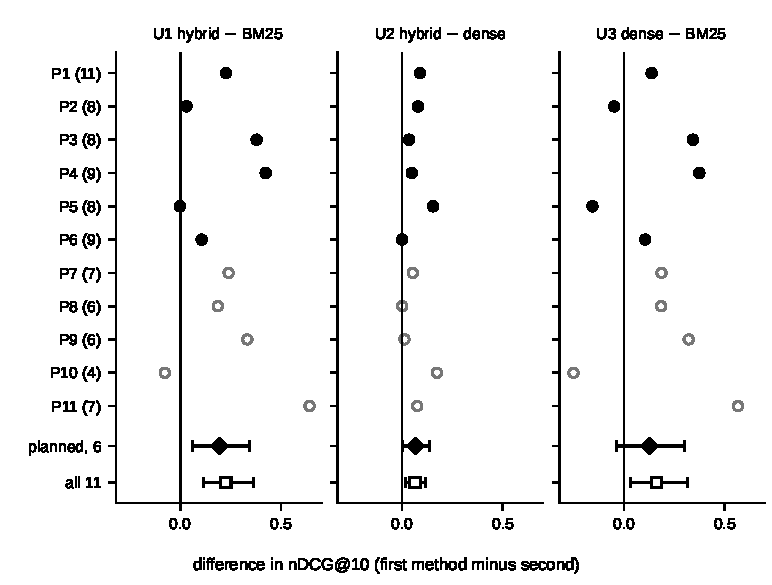
\includegraphics[width=\linewidth]{Fig6.pdf}
\caption{Study 1B: each volunteer's mean paired difference in \ndcg{} (number of scored searches in brackets). Filled circles: the six participants of the planned analysis; open circles: the five with fewer than eight scored searches. Pooled estimates with participant-cluster 95\% intervals: planned analysis (filled diamond) and all eleven participants (open square)}
\label{fig:s1b}
\end{figure}

\paragraph{Analysis.} On the volunteers' phones the three methods come in the same order as on the owner's phone: hybrid 0.901, dense 0.834 and BM25 0.703, against 0.838, 0.787 and 0.584 in Study~1A. The hybrid's lead over BM25 (U1, +0.194) is close to the +0.254 of Study~1A, and its interval excludes zero. It was positive for five of the six analysed participants and essentially zero for P5 ($-$0.002), whose BM25 already found almost everything. The lead over dense search alone (U2, +0.067) is also close to Study~1A's +0.051. Here no analysed participant had a negative mean, and the interval [+0.003, +0.137] just excludes zero. Under the plan neither result is significant. With six participants, the exact test gives $p=0.0625$ as soon as one difference is not positive, and the Holm correction raises this to 0.19. The sensitivity analysis with all eleven volunteers and all 83 scored searches gives the same picture with more weight. Both hybrid gains are significant there (U1 +0.226, Holm $p=0.012$; U2 +0.065, Holm $p=0.006$), and dense search over BM25 (U3, +0.161) narrowly is not ($p=0.055$). Because that analysis includes volunteers whom the plan excludes, we treat it as supporting evidence, not as a confirmatory result.

The volunteers searched mostly for contacts (47 of 106 searches, against 37 file and 22 app searches), whereas the owner's queries in Study~1A were mostly for files, so the two parts weight item types differently. In the planned analysis, BM25 trailed most on files: 0.455, against 0.599 for dense search and 0.703 for the hybrid, over 13 searches. It also trailed on the 7 sentence-like searches: 0.290, against 0.687 and 0.735. On apps, dense search alone was best (0.908, hybrid 0.896; 10 searches), the same pattern as in Study~1A. On contacts the hybrid was best: 0.988, against 0.911 for dense search, over 30 searches. The wanted item appeared in the pooled list for 51 of the 59 searches of the analysed participants. Mean SUS was 82.5 for the six analysed participants and 82.3 for all eleven (range 60 to 100). That is above the mean of about 70 reported across hundreds of SUS studies \citep{bangor2008sus}, but volunteers who know the authors are likely to rate generously.

%=====================================================================
\section{Study 2: speed and cost on phones}\label{sec:s2}

Exact float32 search is fast at personal scale on both phones, but where it becomes slow depends on the phone. Above that point a binary shortlist with rescoring keeps latency low on both, while the app's former LSH configuration loses most true neighbours at every size. On eleven further phones, those of the Study~1B volunteers, the shipped hybrid stayed well under a second per search, and building the index took minutes.

\paragraph{Setup.} Phone~A is the owner's OnePlus CPH2707 (Android 16, 8 cores, Java heap limit 384\,MiB). Phone~B is a group member's Samsung Galaxy M31, SM-M315F (Android 12, 8 cores, heap limit 256\,MiB). Both ran debug builds from clean commits, charging, at thermal status NONE or LIGHT. The vectors are 200,000 MiniLM embeddings of chunks from five BEIR corpora, cut with the app's chunker and shuffled; we test prefixes of $N$ = 10k, 25k, 50k, 100k and 200k on phone~A and 10k, 50k and 100k on phone~B. The queries are 1,000 query vectors from the BEIR query sets, and ground truth is the exact float32 top 10 for each query and $N$. We compared exact float32 search (heap array, or a memory-mapped file from 100k), exact int8 (per-vector symmetric quantisation), a binary shortlist (sign bits, Hamming top $k'=100$ or 200, then float rescoring), the app's LSH index unchanged and with its candidate cap removed, and HNSW (hnswlib-core 1.2.1, $M=16$, efConstruction 200, efSearch 16--128). Each query runs alone on one thread after 50 warm-up queries; we ran three passes of the 1,000 queries and report the median pass. Methods whose estimated heap use would exceed 70\% of the heap limit were skipped. One real-data point on phone~A uses the app's own 13,303 chunk vectors with 200 held-out chunks as queries.

\begin{table}[tbp]
\centering\footnotesize\setlength{\tabcolsep}{3pt}
\caption{Study 2, phone A (OnePlus): recall@10 against exact search / p95 latency (ms) by collection size. A dash marks methods skipped by the heap rule.}
\label{tab:scaling}
\begin{tabular}{lllll}
\toprule
Method & 10k & 50k & 100k & 200k \\
\midrule
Exact float32 & 1.000 / 4.8 & 1.000 / 23.9 & 1.000 / 66.2 & 1.000 / 196.2 \\
Exact int8 & 0.995 / 8.2 & 0.993 / 39.6 & 0.995 / 116.7 & 0.994 / 234.6 \\
Binary + rescore, $k'=100$ & 0.953 / 1.1 & 0.946 / 3.6 & 0.944 / 9.7 & 0.945 / 18.1 \\
Binary + rescore, $k'=200$ & 0.982 / 1.5 & 0.977 / 3.9 & 0.975 / 11.4 & 0.976 / 18.8 \\
LSH, app configuration & 0.055 / 5.4 & 0.034 / 5.7 & 0.029 / 6.3 & -- \\
LSH, uncapped & 0.653 / 14.7 & 0.669 / 50.7 & 0.613 / 74.1 & -- \\
HNSW, efSearch 32 & 0.969 / 1.3 & 0.946 / 1.6 & 0.942 / 2.8 & -- \\
HNSW, efSearch 128 & 0.997 / 3.7 & 0.991 / 4.5 & 0.988 / 7.3 & -- \\
\bottomrule
\end{tabular}
\end{table}

\begin{table}[tbp]
\centering\footnotesize\setlength{\tabcolsep}{3pt}
\caption{Study 2, both phones: p95 latency (ms) and build time at 10k / 50k / 100k vectors. Recall@10 was identical on the two phones for every method (same vectors, deterministic methods).}
\label{tab:devices}
\begin{tabular}{lll}
\toprule
Measure & Phone A: OnePlus CPH2707 & Phone B: Samsung SM-M315F \\
\midrule
Heap limit & 384 MiB & 256 MiB \\
Exact float32, p95 & 4.8 / 23.8 / 66.2 & 12.6 / 61.4 / 208.4 \\
Binary + rescore $k'=200$, p95 & 1.5 / 3.9 / 11.4 & 5.4 / 15.6 / 29.0 \\
Binary + rescore $k'=200$, recall@10 & 0.982 / 0.977 / 0.975 & 0.982 / 0.977 / 0.975 \\
HNSW efSearch 128, p95 & 3.7 / 4.5 / 7.3 & 10.4 / 12.4 / skipped \\
HNSW build (s) & 8.4 / 58.2 / 163.9 & 32.1 / 225.7 / skipped \\
LSH app configuration, recall@10 & 0.055 / 0.034 / 0.029 & 0.055 / 0.034 / 0.029 \\
Exact p95 crosses 50 ms & between 50k and 100k & between 10k and 50k \\
\bottomrule
\end{tabular}
\end{table}

\begin{figure}[tbp]
\centering
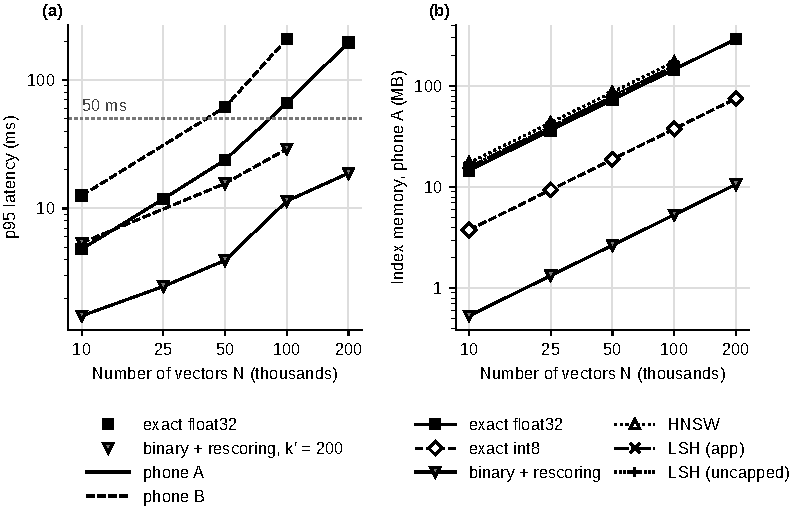
\includegraphics[width=\linewidth]{Fig7.pdf}
\caption{Study 2: (a) p95 latency of exact float32 search (squares) and the binary shortlist with rescoring, $k'=200$ (triangles), against the number of vectors $N$ on both phones (solid lines: phone A; dashed lines: phone B; the dotted horizontal line marks 50\,ms); (b) analytic index memory of each method on phone A, both axes logarithmic. HNSW and the two LSH variants need almost the same memory, so their lines overlap}
\label{fig:latmem}
\end{figure}

\begin{figure}[tbp]
\centering
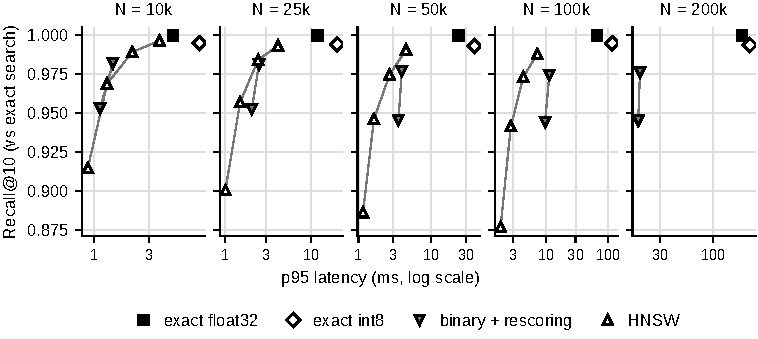
\includegraphics[width=\linewidth]{Fig8.pdf}
\caption{Study 2, phone A: recall@10 against p95 latency for each method and collection size $N$. Thin lines join the settings of one method: efSearch 16, 32, 64 and 128 for HNSW and $k'=100$ and 200 for the binary shortlist (higher settings give higher recall). HNSW was skipped at 200k by the heap rule. Not shown, because they fall far below the axis: the app's LSH configuration (recall@10 0.03--0.06) and LSH without the candidate cap (0.59--0.67)}
\label{fig:recall}
\end{figure}

\paragraph{Analysis.} Four results stand out (Tables~\ref{tab:scaling} and~\ref{tab:devices}, Figures~\ref{fig:latmem} and~\ref{fig:recall}):
\begin{enumerate}
  \item \textbf{Exact search is enough at personal scale, but the limit depends on the phone.} At 50,000 vectors exact float32 search takes 23.9\,ms p95 on phone~A and 61.4\,ms on phone~B, which is 2.6 times slower. Using 50\,ms p95 only as a descriptive marker, phone~A crosses it between 50k and 100k vectors and phone~B between 10k and 50k. At the owner's collection size (about 13,500 vectors) both phones are well below it. The 100k and 200k points ran from a memory-mapped file, which is slower per vector than the heap array.
  \item \textbf{The app's LSH loses most true neighbours.} Its recall@10 was 0.029--0.055 on both phones, and 0.126 on the real-data point. Its low recall is therefore a property of the method, not of the device. Removing the candidate cap raised recall to about 0.6, but latency then grew faster than exact search.
  \item \textbf{The binary shortlist is the cheapest good option at larger $N$.} With $k'=200$ it keeps recall@10 at 0.975--0.982 on both phones and p95 below 30\,ms up to 100k vectors (18.8\,ms at 200k on phone~A). It holds about 11\,MB of bits at 200k; the float vectors stay in the mapped file.
  \item \textbf{HNSW is accurate but costly to build and hold.} It took 164\,s with 8 threads to build at 100k on phone~A and about 175\,MB of heap; on phone~B the build took 226\,s at 50k and did not fit the heap rule at 100k.
\end{enumerate}
Our int8 scan was slower than float32 on Android's runtime (230 vs 193\,ms p50 at 200k); its only benefit here was a fourfold memory saving. These results set the app's switch from exact search to the binary shortlist at 25,000 chunks, below the point where the slower phone reached 50\,ms.

\paragraph{The volunteers' phones.} The eleven Study~1B phones add search latency and index build time on a wider range of hardware (Table~\ref{tab:s1bphones}): Android 11 to 16, 3.5 to 7.4\,GiB of RAM, and collections of 3 to 10,094 chunks. These are end-to-end search times in the study build, recorded for every search; they are not controlled measurements. The shipped hybrid's median latency per phone ranged from 50 to 286\,ms (81.5\,ms at the median and 286\,ms at p95 over all 106 searches). On every phone it was faster at the median than exact dense search alone (57 to 585\,ms), because E2 scans the embeddings stored in the database while E9 scans the in-memory copy (Section~\ref{sec:system}). The slowest phone, P3, holds the largest collection (10,094 chunks), and its p95 of 1,505\,ms rests on nine searches.

\begin{table}[tbp]
\centering\footnotesize\setlength{\tabcolsep}{3pt}
\caption{Study 2: the eleven Study 1B phones (labels as in Table~\ref{tab:s1bpart}). Build: one index build per phone, from start to end as recorded in the export, under uncontrolled conditions. Units: RAM in GiB, build in minutes, battery in percent at start and end, latency in ms (median over that participant's searches, rounded to whole ms; p95 for E9 only).}
\label{tab:s1bphones}
\begin{tabular}{llrrrrlrrrr}
\toprule
 & Phone & Android & RAM & Chunks & Build & Battery & E1 & E2 & E9 & E9 p95 \\
\midrule
P1 & SM-M315F & 12 & 7.4 & 1,715 & 15.4 & 81 $\to$ 81\footnotemark[2] & 44 & 320 & 258 & 280 \\
P2 & 25057RN09I & 16 & 5.3 & 44 & 0.3 & 18 $\to$ 18 & 18 & 85 & 65 & 88 \\
P3 & SM-A515F & 13 & 5.4 & 10,094 & 413.5\footnotemark[1] & 52 $\to$ 100\footnotemark[2] & 72 & 585 & 286 & 1,505 \\
P4 & POCO M2 Pro & 12 & 3.5 & 2,509 & 4.9 & 73 $\to$ 72 & 46 & 127 & 84 & 91 \\
P5 & moto g45 5G & 15 & 7.3 & 438 & 1.8 & 46 $\to$ 46 & 18 & 57 & 52 & 59 \\
P6 & 22031116AI & 13 & 5.5 & 77 & 0.3 & 31 $\to$ 31 & 18 & 169 & 145 & 217 \\
P7 & 22111317PI & 14 & 7.3 & 2,834 & 5.8 & 84 $\to$ 82 & 30 & 92 & 69 & 80 \\
P8 & SM-A146B & 15 & 7.3 & 738 & 2.5 & 68 $\to$ 67 & 24 & 88 & 50 & 81 \\
P9 & I2018 & 13 & 7.2 & 3 & 1.1 & 99 $\to$ 99 & 44 & 101 & 99 & 147 \\
P10 & moto g86 power 5G & 16 & 7.2 & 66 & 0.6 & 92 $\to$ 92\footnotemark[2] & 17 & 67 & 61 & 65 \\
P11 & Redmi Note 8 Pro & 11 & 5.5 & 7,707 & 15.8 & 63 $\to$ 58 & 81 & 225 & 100 & 148 \\
\bottomrule
\end{tabular}
\footnotetext[1]{See text.}
\footnotetext[2]{Plugged in for the whole build (P2 was plugged in only at the end).}
\end{table}

\paragraph{Index build time.} Building the index took 0.3 to 15.8 minutes on ten of the eleven phones, including 7,707 chunks in 15.8 minutes on the phone with the oldest Android version (P11, Android 11). The exception is P3: 413.5 minutes for 10,094 chunks, while the phone charged from 52 to 100\%. The export records only the start and end of the build, so we cannot tell how long Android paused or throttled the background work. A collection of similar size took 15.8 minutes on P11, so we report the P3 value but do not treat it as the cost of indexing. Unplugged builds used at most 5 percentage points of battery (P11).

\paragraph{Release-mode check.} We repeated part of the measurement on phone~A with a non-debuggable benchmark build (R8 off). Table~\ref{tab:release} shows the full-search latency.

\begin{table}[tbp]
\centering\footnotesize\setlength{\tabcolsep}{3pt}
\caption{End-to-end search latency on phone A, debug build versus non-debuggable benchmark build (64 Set~A queries $\times$ 5 repetitions, thermal NONE). Rankings were identical in all 640 (arm, query, repetition) pairs.}
\label{tab:release}
\begin{tabular}{lccc}
\toprule
Arm & Debug, median / p95 (ms) & Benchmark build, median / p95 (ms) & Change \\
\midrule
E9 (shipped) & 122.0 / 178.1 & 94.0 / 140.1 & $-$23\% / $-$21\% \\
E12 (pre-study) & 92.0 / 131.2 & 78.0 / 110.1 & $-$15\% / $-$16\% \\
\bottomrule
\end{tabular}
\end{table}

\paragraph{Analysis.} The build type changes speed only, never the ranking. The latencies reported elsewhere in this paper come from debug builds and are therefore conservative. In the scaling subset at 10k and 50k vectors, the binary shortlist and HNSW ran 1.5--2.7 times faster without the debuggable runtime; the float scan showed no consistent difference, because thermal spread was as large as any build effect.

\paragraph{Resource use.} Table~\ref{tab:resources} gives the storage and memory footprint of version 1.0.0. The release bundle is 353\,MB because it carries the CLIP image-search models as a separate asset pack (two fp16 models, 303\,MB as stored in the repository); without that pack the universal APK built from the bundle is 81\,MB, of which the two text models are 68\,MB. For memory, an instrumented test ran 20 searches (the five generic queries four times) through the shipped configuration on phone~A and read the process's own memory (\texttt{Debug.MemoryInfo}) at start, after one warm-up search and after the 20 searches; it was repeated three times.

\begin{table}[tbp]
\centering\footnotesize\setlength{\tabcolsep}{3pt}
\caption{Study 2, resource use of version 1.0.0 (sizes in MB = $10^6$ bytes). Memory: phone A, debug build, 14,886 chunks indexed, three runs (range); PSS is the proportional set size of the app process.}
\label{tab:resources}
\begin{tabular}{lr@{\hspace{2.5em}}lr}
\toprule
Storage & MB & Process memory (20 searches) & MB \\
\midrule
Release bundle (AAB) & 352.8 & Total PSS at start & 218--225 \\
Universal APK (no CLIP pack) & 81.0 & Total PSS after warm-up & 1,164--1,207 \\
MiniLM text encoder & 22.7 & Total PSS after 20 searches & 1,024--1,029 \\
Cross-encoder (off by default) & 45.3 & Java heap after 20 searches & 53--58 \\
CLIP models (asset pack, fp16) & 302.9 & Native heap after 20 searches & 608--614 \\
 & & In-memory dense index (float32) & 22.9 \\
\bottomrule
\end{tabular}
\end{table}

\paragraph{Analysis.} The search itself adds little to the footprint: the in-memory dense index for 14,886 chunks is 22.9\,MB. Most of the roughly 1\,GB of PSS after warm-up is native memory, which we did not break down; it includes the loaded models and their runtime buffers. PSS fell by 140--180\,MB between the warm-up search and the end of the run and, in the run we logged round by round, stayed within 4\,MB over the last three rounds, so we saw no growth over 20 searches, but 20 searches is a short run and the figure is for a debug build on one phone, measured inside the instrumentation process (which also holds the test classes). The collection had grown to 14,886 chunks since Study~1 (13,696). Energy was measured as battery charge used per 100 searches above the idle drain over the same time: a median of 2.9\,mAh per 100 searches (2.7--3.5\,mAh over three repeats of 600 searches each). The conditions were one phone, a debug build, screen on at about half brightness and searches run back to back; idle drain varied between the repeats (36--73\,mAh per 10 minutes), so the figure is an order of magnitude rather than a precise cost.

%=====================================================================
\section{Study 3: replication on public data}\label{sec:s3}

On five public datasets, exact search beat LSH in the hybrid every time, reranking again made no detectable difference, and no embedding model won everywhere.

\paragraph{Method.} We ported the app pipeline to Python (Figure~\ref{fig:replication}). The chunker, query processing, the LSH index (bit-identical tables and search results) and both fusion functions are tested against fixtures produced by the Kotlin code. BM25 uses the same FTS5 table definition and SQL. MiniLM and the cross-encoder are the PyTorch versions of the models the app ships in TensorFlow Lite. We ran nine configurations on the BEIR test sets of SciFact, NFCorpus, FiQA-2018, SCIDOCS and TREC-COVID \citep{thakur2021beir} (300, 323, 648, 1,000 and 50 queries). The analysis plan was committed to the repository before any result was computed. It fixed four contrast families: C1 exact vs LSH in the RRF hybrid; C2 RRF vs global normalisation; C3 reranking the top 20; and C4 each alternative embedder vs MiniLM in the hybrid. We used paired randomisation tests over queries (10,000 sign flips) with Holm correction over all 38 executed contrast--dataset pairs. The study is exploratory: planned, but not pre-registered. With 10,000 permutations the smallest possible Holm-adjusted $p$ is 0.0038.

\begin{figure}[tbp]
\centering
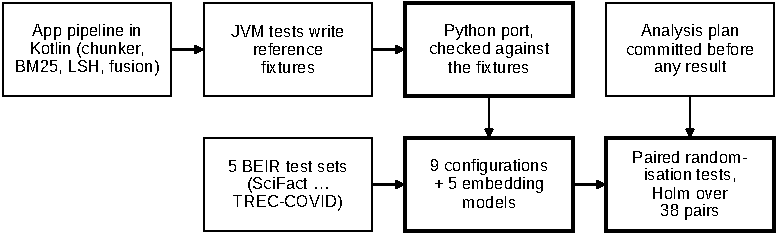
\includegraphics[width=\linewidth]{Fig9.pdf}
\caption{Study 3 workflow: a Python port of the app pipeline, checked against fixtures written by the Kotlin code, run on five public BEIR datasets under an analysis plan committed before any result}
\label{fig:replication}
\end{figure}

\paragraph{Fidelity check.} Our BM25 follows the app's AND-to-OR cascade, not a standard BEIR BM25 run. It scores close to the published BEIR BM25 \citep{thakur2021beir} on SciFact (0.661 vs 0.665) and SCIDOCS (0.155 vs 0.158), lower on NFCorpus (0.288 vs 0.325) and FiQA (0.211 vs 0.236), and much lower on TREC-COVID (0.507 vs 0.656).

\begin{table}[tbp]
\centering\footnotesize\setlength{\tabcolsep}{3pt}
\caption{Study 3: \ndcg{} per configuration (MiniLM). Bold marks the best configuration per dataset.}
\label{tab:beir}
\begin{tabular}{lccccc}
\toprule
Configuration & SciFact & NFCorpus & FiQA & SCIDOCS & TREC-COVID \\
\midrule
BM25 & 0.661 & 0.288 & 0.211 & 0.155 & 0.507 \\
Dense exact & 0.628 & 0.292 & \textbf{0.377} & \textbf{0.205} & 0.599 \\
Dense LSH & 0.164 & 0.075 & 0.040 & 0.037 & 0.250 \\
Dense int8 & 0.628 & 0.292 & 0.377 & 0.205 & 0.600 \\
Dense binary + rescore & 0.627 & 0.288 & 0.373 & 0.205 & 0.602 \\
Hybrid RRF, exact (E9) & 0.676 & 0.324 & 0.334 & 0.196 & 0.655 \\
Hybrid RRF, LSH (E5) & 0.478 & 0.260 & 0.161 & 0.116 & 0.442 \\
Hybrid global normalisation, exact & \textbf{0.692} & 0.317 & 0.323 & 0.192 & \textbf{0.666} \\
Hybrid RRF, exact + rerank 20 (E10) & 0.666 & \textbf{0.327} & 0.331 & 0.197 & 0.664 \\
\bottomrule
\end{tabular}
\end{table}

\begin{table}[tbp]
\centering\footnotesize\setlength{\tabcolsep}{3pt}
\caption{Study 3: planned contrasts C1--C3 per dataset: C1 exact minus LSH dense search in the RRF hybrid, C2 RRF minus global score normalisation, C3 reranking the top 20 minus no reranking (difference in \ndcg{}, Holm-adjusted $p$ over 38 pairs in brackets).}
\label{tab:beircontrasts}
\begin{tabular}{lccccc}
\toprule
Contrast & SciFact & NFCorpus & FiQA & SCIDOCS & TREC-COVID \\
\midrule
C1 exact $-$ LSH & +0.198 (0.004) & +0.064 (0.004) & +0.173 (0.004) & +0.081 (0.004) & +0.212 (0.004) \\
C2 RRF $-$ global & $-$0.016 (0.29) & +0.007 (0.28) & +0.012 (0.04) & +0.005 (0.12) & $-$0.012 (1.00) \\
C3 rerank $-$ none & $-$0.010 (1.00) & +0.004 (1.00) & $-$0.003 (1.00) & +0.001 (1.00) & +0.009 (1.00) \\
\bottomrule
\end{tabular}
\end{table}

\paragraph{Analysis.} Table~\ref{tab:beircontrasts} answers the three pipeline questions on public data. C1 replicates the direction of Set~B's H1 on every dataset, with larger effects (+0.064 to +0.212), because on these corpora the dense half carries more of the ranking and LSH loses most of its neighbours (dense LSH reaches 0.04--0.25 against 0.21--0.63 for exact dense search). C3 replicates Set~B's H4: reranking the top 20 changes \ndcg{} by at most 0.010 in either direction. C2 shows no consistent winner between RRF and global normalisation; only FiQA is significant (+0.012 for RRF). Two descriptive points complete the picture. The hybrid beat exact dense search on SciFact, NFCorpus and TREC-COVID but not on FiQA or SCIDOCS, so the benefit of adding BM25 depends on the collection. And quantisation is almost free: int8 stayed within 0.001 \ndcg{} of exact float32 and the binary shortlist within 0.004.

\begin{table}[tbp]
\centering\footnotesize\setlength{\tabcolsep}{3pt}
\caption{Study 3: \ndcg{} of the hybrid RRF exact configuration with each embedder (C4). An asterisk marks a Holm-significant difference from MiniLM.}
\label{tab:embedders}
\begin{tabular}{lrrrccccc}
\toprule
Model & Params & Dim. & Chunks/s\footnotemark[1] & SciFact & NFCorpus & FiQA & SCIDOCS & TREC-COVID \\
\midrule
MiniLM-L6 (app) & 22.7M & 384 & -- & 0.676 & 0.324 & 0.334 & 0.196 & 0.655 \\
bge-small & 33.4M & 384 & 162 & 0.702 & 0.346$^{*}$ & 0.335 & 0.192 & 0.729$^{*}$ \\
arctic-embed-xs & 22.6M & 384 & 285 & 0.680 & 0.326 & 0.303$^{*}$ & 0.183$^{*}$ & 0.743$^{*}$ \\
potion-base-8M & 7.6M & 256 & 11,644 & 0.614$^{*}$ & 0.298$^{*}$ & 0.207$^{*}$ & 0.152$^{*}$ & 0.548$^{*}$ \\
EmbeddingGemma & 307.6M & 768 & 34 & 0.730$^{*}$ & 0.362$^{*}$ & 0.359$^{*}$ & 0.185$^{*}$ & -- \\
EmbeddingGemma & 307.6M & 256 & --\footnotemark[2] & 0.732$^{*}$ & 0.357$^{*}$ & 0.362$^{*}$ & 0.185$^{*}$ & -- \\
\bottomrule
\end{tabular}
\footnotetext[1]{Encoding throughput on the laptop, from a 512-chunk sample; not a phone measurement. EmbeddingGemma was not run on TREC-COVID (time budget).}
\footnotetext[2]{Derived by truncating the 768-dimension vectors (Matryoshka), so it has no separate throughput.}
\end{table}

\begin{figure}[tbp]
\centering
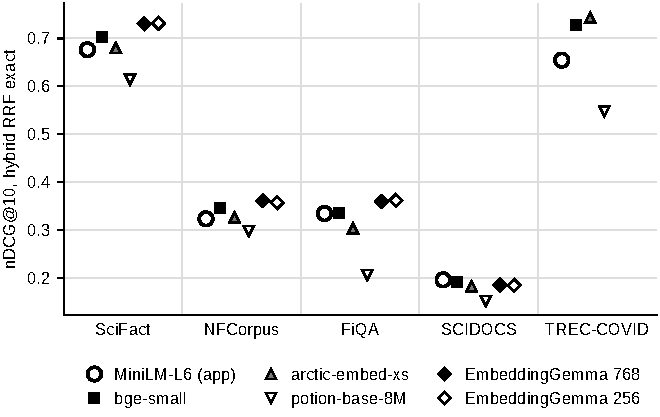
\includegraphics[width=\linewidth]{Fig10.pdf}
\caption{Study 3: \ndcg{} of the hybrid RRF exact configuration with each embedder on the five BEIR datasets. MiniLM (large open circle) is the model the app ships. EmbeddingGemma was not run on TREC-COVID}
\label{fig:embedders}
\end{figure}

\paragraph{Analysis of the embedders.} No small model won everywhere (Table~\ref{tab:embedders}, Figure~\ref{fig:embedders}). Compared with MiniLM in the hybrid, EmbeddingGemma-300M was better on SciFact (+0.054), NFCorpus (+0.038) and FiQA (+0.025) and worse on SCIDOCS ($-$0.011), all Holm $p \le 0.0042$; truncated to 256 dimensions it stayed within 0.005 of its 768-dimension score. bge-small was better on NFCorpus (+0.022) and TREC-COVID (+0.074); arctic-embed-xs was better on TREC-COVID (+0.089) and worse on FiQA and SCIDOCS; the static Model2Vec potion-base-8M was worse everywhere ($-$0.025 to $-$0.128). Cost differs by orders of magnitude: EmbeddingGemma encoded 34 chunks/s on the laptop sample and potion-base-8M 11,644. The alternatives used 256 tokens and no cosine floor, while MiniLM kept the app's 128 tokens and 0.3 floor, so C4 compares the models as configured, not under identical settings.

%=====================================================================
\section{Discussion}

Studies~1 to 3 agree on one practical message: at the size of a personal collection, approximate hashing saves almost nothing and costs quality, while exact search is cheap.

\paragraph{The hybrid earns its place, mostly against BM25.} On the owner's phone the hybrid beat BM25 by 0.254 \ndcg{}; its gain over exact dense search alone was smaller (+0.051) and not significant, and on public data the hybrid beat dense search on three of five datasets and lost on two. We still ship the hybrid for two reasons. BM25 finds exact names (apps, contacts, file titles) that dense search can miss, and dense search finds paraphrases that BM25 misses; and the hybrid was never significantly worse than dense search on the phone, while fusion adds only milliseconds. Study~1B points the same way: on the volunteers' phones the hybrid led dense search by +0.067, with an interval just above zero but not significant under its plan. Taken together, the two parts suggest that the gain over dense search alone is real but small, around 0.05 to 0.07 \ndcg{}, which is close to what either part can detect on its own. A larger registered multi-user study is needed to confirm it.

\paragraph{Other people's phones agree with the owner's.} Study~1B is small and was not registered, but where it overlaps with Study~1A it agrees. The hybrid led BM25 by about 0.2 \ndcg{} on the volunteers' phones, against 0.25 on the owner's and its lead over dense search was zero or positive for every analysed volunteer. The volunteers' data also showed two things Study~1A could not. Several phones held only a handful of documents, so most searches were for contacts and apps, where all three methods did well and the hybrid mainly helped on contacts. And on ordinary phones indexing up to about 7,700 chunks took at most 16 minutes, apart from one build that was slowed for reasons we cannot see, while each search took well under a second.

\paragraph{Exact before approximate.} Study~2 puts exact float32 search at 4.8 to 12.6\,ms p95 for 10,000 vectors on the two phones; a typical phone collection like ours (13,500 vectors) sits well inside an interactive budget on both. The LSH configuration, tuned for speed, kept 3--13\% of the true neighbours, and Study~3 shows what that costs on public data: 0.06--0.21 \ndcg{} in the hybrid. On the personal collection the cost inside the hybrid was smaller (+0.044 for exact) and not significant at the cluster level, likely because BM25 and the exact scans of apps and contacts covered for the dense half on name-like queries; on sentence-like queries the stratum estimate was +0.168. An approximate index should be the exception, adopted only when exact search is measured to be too slow.

\paragraph{Beyond a few tens of thousands of vectors.} If a collection grows past what exact search serves in time, a binary shortlist with float rescoring was the best trade-off we measured: below 30\,ms p95 up to 100,000 vectors on both phones, no build step beyond packing sign bits, about 11\,MB at 200,000 vectors, and at most 0.004 \ndcg{} lost end to end. HNSW was more accurate per millisecond, but its build time (164\,s at 100,000 vectors on the faster phone, 226\,s at 50,000 on the slower one) and heap use are costly on a phone that must re-index in the background. Because the point where exact search slows down differs between phones by more than a factor of two, LocalSeek~1.0.0 switches to the binary shortlist at 25,000 chunks, a threshold set from the slower phone.

\paragraph{Fusion details matter as much as models.} The largest registered gain from a single setting was the change from one min-max scale over three FTS5 tables to a rank-based merge (+0.105). Raw BM25 scores from different tables are not comparable, so one scale lets one table crowd out the others, a property of multi-source personal search that web benchmarks do not exercise. Between RRF and global normalisation for the hybrid itself, Study~3 found small differences whose direction changed by dataset. \citet{bruch2023fusion} showed that a tuned convex combination can beat RRF; we tuned neither function, so our result says only that the untuned defaults differ little.

\paragraph{Reranking did not pay on the phone.} A 22M-parameter cross-encoder over the top 20 took about 4.8\,s per query and showed no detectable gain in Study~1 or on any public dataset. The registered cascade kept the reranker's quality at 29\% lower mean latency but could not show a gain over not reranking at all.

\paragraph{The embedding model is the open lever.} No small model won everywhere. EmbeddingGemma gained 0.025--0.054 \ndcg{} on three of four datasets and lost on one; it is about 14 times larger than MiniLM and about 340 times slower than the static Model2Vec model on our laptop sample, though its 256-dimension truncation kept nearly all of the gain. Changing the shipped encoder needs a re-index and phone-side latency measurements we have not yet made.

\paragraph{Shipping what was measured.} The configuration shipped before this study was 0.147 \ndcg{} below the best one we had, mostly on apps and contacts. Because the arms were explicit configuration objects with recorded hashes, switching the app to the measured configuration was a small change guarded by tests. We recommend this practice to other on-device search projects.

%=====================================================================
\section{Limitations and threats to validity}\label{sec:limits}

\paragraph{Assessors.} In Study~1A one assessor wrote the queries, owns the data and judged the results, and judging was fast (about 1\,s per row). Self-agreement was measured on a blind re-judge of 8 queries (Cohen's $\kappa=0.69$, Section~\ref{sec:s1method}), but agreement between different assessors was not. In Study~1B each volunteer judged their own lists once, so agreement between assessors is again unmeasured, and the volunteers are peers of the authors rather than a sample of users. Results may not transfer to other people's collections or query habits.

\paragraph{Study~1B is small and not registered.} Six volunteers met the planned minimum of eight scored searches (53 searches). The other five, with 4 to 7 scored searches each, enter only the sensitivity analysis. No contrast reached significance under the plan; the significant hybrid gains come from the sensitivity analysis, which was not planned. Four phones held 11 or fewer indexed files. Pooled judging only covers items that one of the three methods returned, so absolute \ndcg{} is optimistic and only the contrasts are meaningful. The plan was committed to the repository before any participant file existed but not registered on OSF.

\paragraph{Power.} With 64 clusters the minimum detectable effect is about 0.06--0.07 \ndcg{}; the nulls for H1, H2 and H4 (and the hybrid-vs-dense contrast) are not evidence of equality, and the sentence-like stratum (17 clusters) is descriptive only.

\paragraph{The pilot was seen.} The confirmatory hypotheses were shaped by Set~A, as disclosed in the registration. In Set~A the one significant hybrid result (rerank vs hybrid, Holm $p=0.024$ by query) weakens to $p=0.066$ when clusters are respected.

\paragraph{Pooling depth.} Only the top 10 of each arm was judged; 18--31\% of each arm's top 20 is unjudged, so deeper metrics are not reported.

\paragraph{Measurement.} Study~1 and most of Study~2 ran on debuggable builds; a release-mode check lowered E9's median latency from 122 to 94\,ms with identical rankings, so the reported latencies are conservative. Study~2 used two phones, one session each, with different heap limits (384 vs 256\,MiB) and Android versions, so latency differences between them are not attributed to a single cause. The battery level at build time could shrink the former LSH index (5 tables and a cap of 70 when rebuilt at 20--49\% battery), a confound the Set~B run controlled by rebuilding at high charge. Study~2 timed the dense index alone; the 100k and 200k exact points used a memory-mapped file; HNSW and LSH at 200k (and HNSW at 100k on phone~B) were skipped by the heap rule; our int8 scan is a plain Kotlin loop without SIMD; and the exact scan over the real chunk vectors was slower than the public-vector trend predicts (9.4 vs about 6.3\,ms p95) for a reason we could not find.

\paragraph{Replication fidelity.} Study~3 uses PyTorch MiniLM instead of the app's TensorFlow Lite model and a desktop SQLite build; our BM25 follows the app's query cascade and scores below standard BM25 on three datasets; the embedder comparison mixes token limits (128 vs 256) and cosine floors; EmbeddingGemma was not run on TREC-COVID; and public science, finance and COVID texts differ from personal files.

\paragraph{Not measured.} Energy over a normal day of use (it was measured only for back-to-back searches, Section~\ref{sec:s2}), memory under pressure from other apps, and image search. Process memory was measured on one phone, in a debug build, for 20 searches only (Section~\ref{sec:s2}). Index build time was recorded only as a by-product of Study~1B (one build per phone, no controlled conditions).

%=====================================================================
\section{Conclusion}

On one person's phone, the measured best configuration of an on-device hybrid search engine beat the shipped one by 0.147 \ndcg{} with simpler machinery: exact dense search, rank fusion, and no reranking, diversification or dense skipping. Across a pre-registered on-device study, a scaling benchmark on two phones and a replication on five public datasets, three findings held: exact search is fast enough at personal scale, though the size where it slows down differs by phone, while LSH loses quality; merging ranks rather than raw scores across sources matters; and a cross-encoder reranker does not pay for its latency. On eleven volunteers' own phones the hybrid again led BM25 by about 0.2 \ndcg{} and dense search by a small margin; both gains were significant only in a sensitivity analysis that kept every volunteer. LocalSeek~1.0.0 ships these findings. The open questions are the embedding model and a second assessor. The next step is a larger, registered multi-user study with larger collections, under the same aggregate-only privacy rules.

\backmatter

\bmhead{Acknowledgements}
The authors are grateful to their project guide, Prof.\ Pallavi Thakur, Sardar Patel Institute of Technology, Mumbai, for her guidance and supervision throughout this work. The authors also thank the volunteers who took part in the user study.

\section*{Statements and Declarations}

\bmhead{Funding} No funding was received for conducting this study.

\bmhead{Competing interests} The authors have no competing interests to declare that are relevant to the content of this article.

\bmhead{Ethics approval and consent to participate} The user study (Study 1B) was approved by Sardar Patel Institute of Technology, Mumbai. All volunteers gave informed consent on a consent screen in the study app before any data were recorded. The app recorded only numbers and categories; no search text, file names, contact names or other personal content left the volunteers' phones. Study 1A used only the first author's own phone and data.

\bmhead{Consent for publication} Not applicable: the article contains no identifying information about any person.

\bmhead{Data availability} The public datasets of Study 3 are the BEIR test collections \cite{thakur2021beir}. Per-query results for Study 3, the aggregate results of Studies 1 and 2 and the aggregate user-study results are in the project repository (\url{https://github.com/greenaltambe/LocalSeek}). The Study 1A queries, judgments and collection, and the per-participant exports of Study 1B, contain or derive from personal data and are not shared; the Study 1A registration is public at \url{https://osf.io/vwmfz}.

\bmhead{Code availability} The app, benchmark harness and analysis code are open source at \url{https://github.com/greenaltambe/LocalSeek}.

\bibliography{references}

\end{document}
